\documentclass[12pt, a4paper]{article}
\usepackage{titlesec}
\usepackage{graphicx}
\usepackage{amsmath}
\renewcommand{\figurename}{Att.}
\titlelabel{\thetitle.\quad}
\author{Pēteris Račinskis pr20015}
\date{05/12/21}
\begin{document}
\title{4. mājas darbs}

\maketitle

\section{Uzdevums}

Dots koka $G$ Prūfera kods $P=(1,1,3,3,1,8,5,7)$. Atjaunoto koku $G' = (V',E')$ var iegūt, paplašinot kodu ar maksimālo elementu
\begin{equation}
    V'_0 = \lbrace P_{n-1} \rbrace = \lbrace \max(V[G]) \rbrace; E'_0=\emptyset
\end{equation}
un ar $i=\lbrace 1, ..., n-2 \rbrace$ izpildot soļus
\begin{equation}
    v_i = 
\begin{cases}
    P_{n-i-1}, \text{ ja } P_{n-i-1} \notin V'_{i-1} \\
    \max(V[G] \setminus V_{i-1})
\end{cases}
\end{equation}
\begin{equation}
    V'_i = V'_{i-1} \cup v_i
\end{equation}
\begin{equation}
    E'_i = E'_{i-1} \cup \lbrace v_i, P_{n-i} \rbrace
\end{equation}
Process attēlots grafiski:

\begin{figure}[h!]
    \centering
    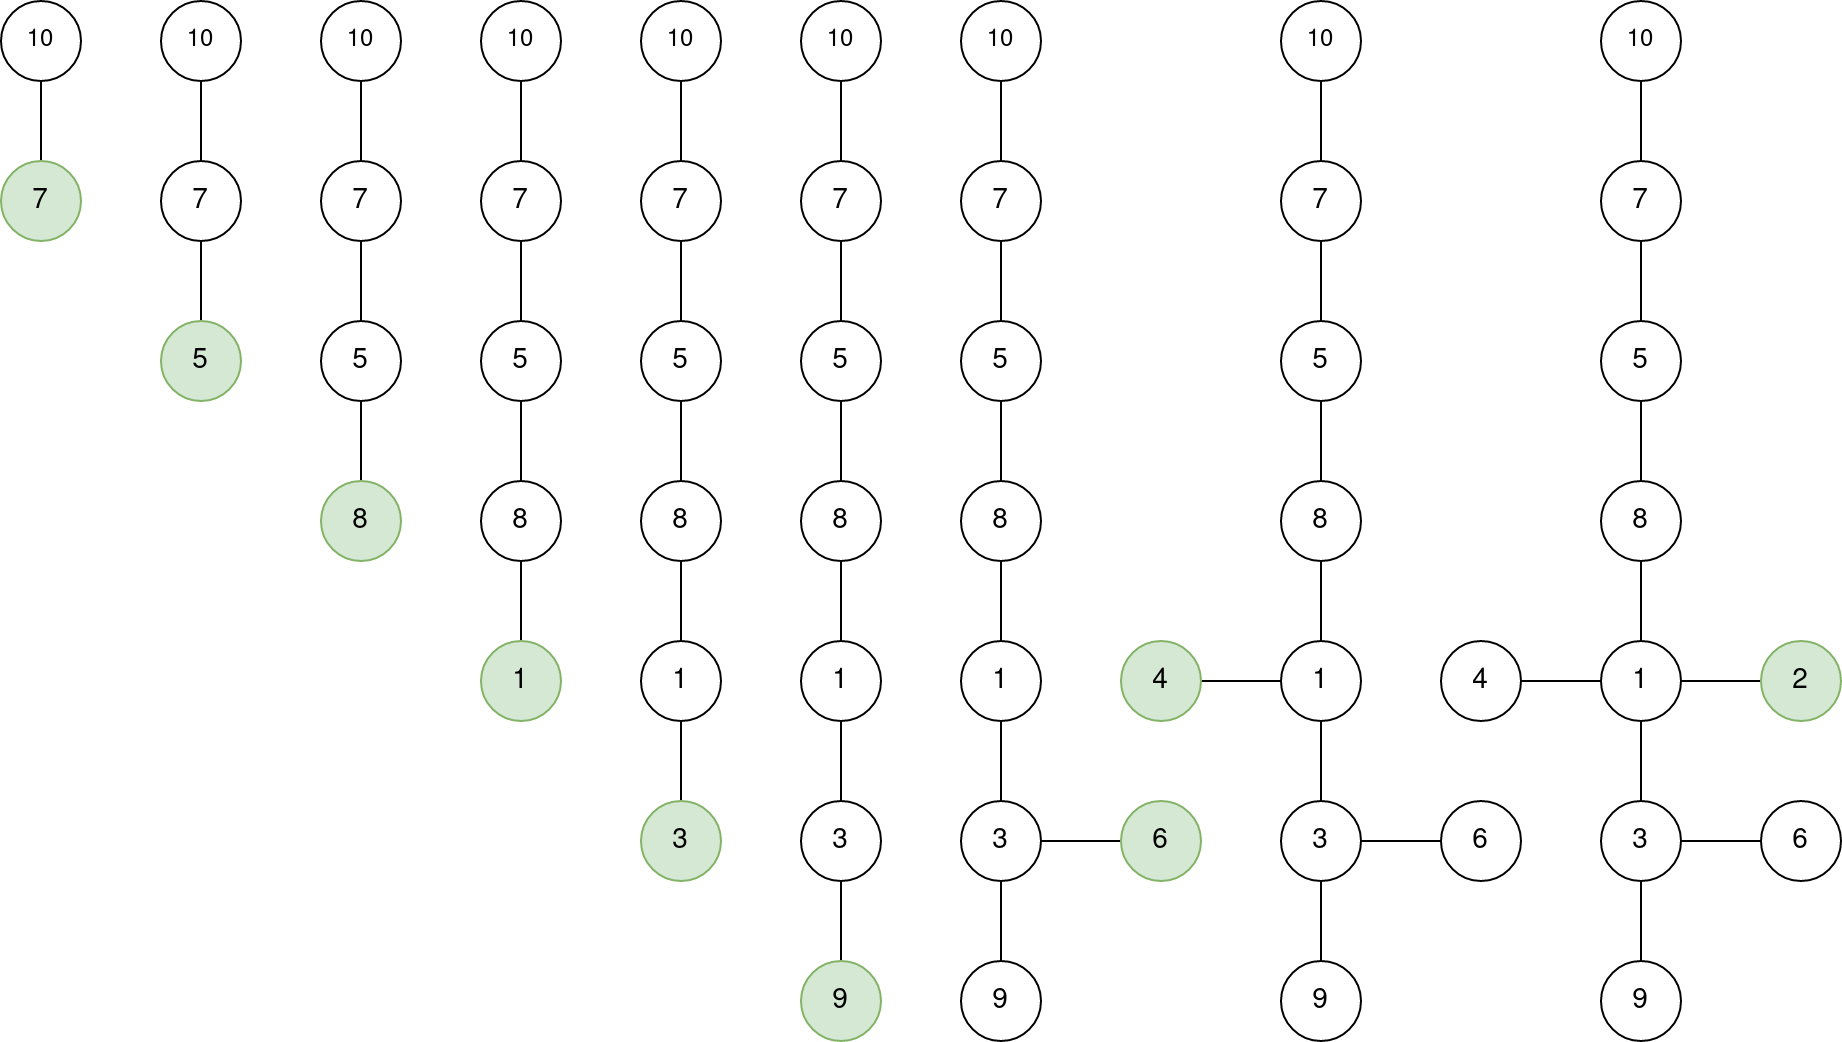
\includegraphics[height=5.5cm,page=1]{pruefer.png}
    \caption{Koka atjaunošana pēc Prūfera koda.}
\end{figure}

\newpage
\section{Uzdevums - NAV PAREIZI, ŠĶAUTNES}

\begin{figure}[h!]
    \centering
    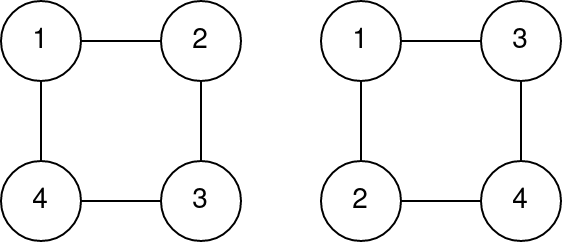
\includegraphics[height=4cm]{vertex-order.png}
    \caption{Izomorfi grafi ar dažādu virsotņu secību ciklā.}
\end{figure}


Ciklu matrica nesniedz nekādu informāciju par virsotņu secību ciklā. Abiem 2. attēlā redzamajiem grafiem ir tā pati ciklu matrica 
$$C=\begin{bmatrix}
    1 & 1 & 1 & 1
\end{bmatrix}$$

, bet grafi ir dažādi, jo $E[G_1] \triangle E[G_2] = \lbrace
\lbrace 1, 4\rbrace,
\lbrace 1, 3\rbrace,
\lbrace 2, 3\rbrace,
\lbrace 2, 4\rbrace
\rbrace$, lai arī izomorfi. Šī īpašība ļauj arī grafiem, kas pieder dažādām izomorfismu klasēm, būt vienādām ciklu matricām. 3. attēlā starp grafiem izomorfisms nepastāv, jo tikai vienam no tiem $\exists e = \lbrace u, v \rbrace \in E[G] : \deg(u) = \deg(v) = 4 $, kaut gan abos gadījumos ciklu matrica ir $$ 
C=\begin{bmatrix}
    1 & 1 & 1 & 1 & 0 & 0 & 0 & 0 \\
    0 & 1 & 0 & 0 & 1 & 1 & 0 & 0 \\
    0 & 0 & 0 & 1 & 0 & 0 & 1 & 1 \\
    
\end{bmatrix}
$$

\begin{figure}[h!]
    \centering
    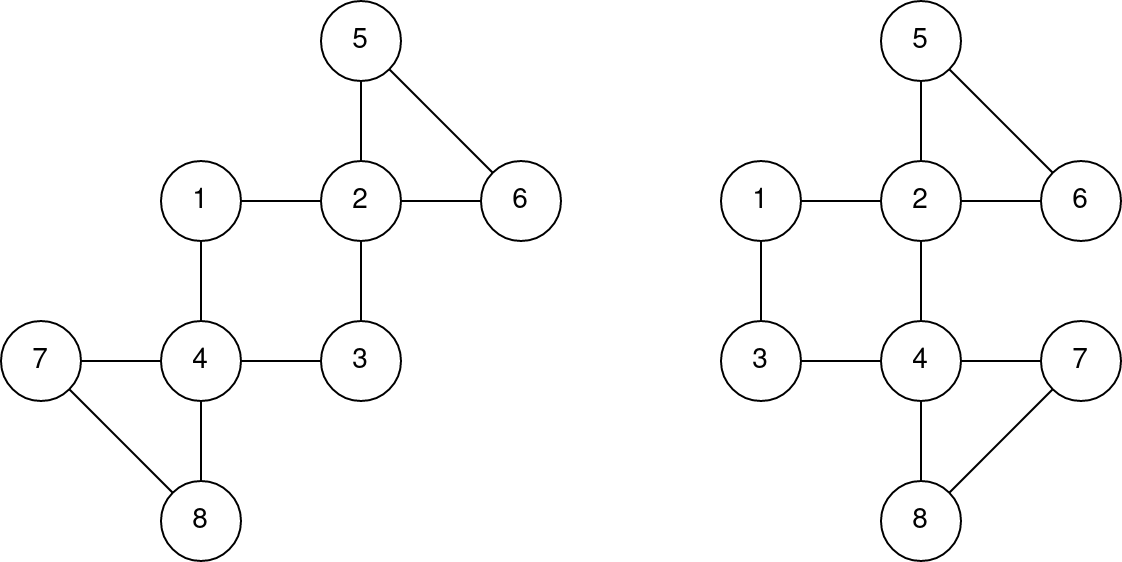
\includegraphics[height=5cm]{not-isomorphic.png}
    \caption{Ne-izomorfi grafi ar dažādu virsotņu secību ciklā.}
\end{figure}

\newpage
\section{Uzdevums}

Izmantojot formulu ciklomātiskā skaitļa aprēķinam
\begin{equation}
    r(G) = m-n+k
\end{equation}
var pierādīt dažādu modifikāciju izraisītās izmaiņas.

\subsection{Virsotnes pievienošana uz malas}
Formāli doto modifikāciju $f(V[G], E[G], e)=(V',E')=G'$ var izteikt kā
\begin{equation}
    e= \lbrace u,v \rbrace \in E[G]
\end{equation}

\begin{equation}
    f(V,E,e) = (V \cup w, (E \setminus \lbrace u,v \rbrace) \cup \lbrace
    \lbrace u,w \rbrace, \lbrace w,v \rbrace 
    \rbrace)
\end{equation}
no kā izriet, ka
\begin{equation}
    \vert V' \vert = \vert V \vert + 1 = n + 1
\end{equation}
\begin{equation}
    \vert E' \vert = \vert E \vert -1 + 2 = m + 1
\end{equation}
\begin{equation}
    u,v \in K_i \text{ komponentē} \rightarrow u,w,v \in K'_i
\end{equation}
tātad
\begin{equation}
    r(G') = (m+1)-(n+1)+k = m-n+k = r(G)
\end{equation}


\subsection{Virsotnes ar pakāpi = 2 aizstāšana ar šķautni}
Turpinot pēc analoģijas
\begin{equation}
    w \in V[G] : \deg(v) = 2 \rightarrow \lbrace u,w \rbrace, \lbrace w,v \rbrace \in E[G]
\end{equation}
\begin{equation}
    f(V,E,w) = (V \setminus w, (E \setminus \lbrace \lbrace u,w \rbrace, \lbrace w,v\rbrace  \rbrace) \cup \lbrace u,v \rbrace)
\end{equation}
\begin{equation}
    \vert V' \vert = \vert V \vert - 1 = n - 1
\end{equation}
\begin{equation}
    \vert E' \vert = \vert E \vert - 2 + 1 = m - 1
\end{equation}
\begin{equation}
    u,w,v \in K_i \text{ komponentē} \rightarrow u,v \in K'_i
\end{equation}
tātad
\begin{equation}
    r(G') = (m-1)-(n-1)+k = m-n+k = r(G)
\end{equation}

\newpage
\subsection{Virsotnes ar pakāpi = 1 izgriešana}
Paša definētā modifikācija - visvienkāršākā. Nogriež lapu.

\begin{equation}
    w \in V[G] : \deg(v) = 1 \rightarrow \lbrace u,w \rbrace \in E[G]
\end{equation}
\begin{equation}
    f(V,E,v) = (V \setminus w, E \setminus \lbrace u,w \rbrace)
\end{equation}
\begin{equation}
    \vert V' \vert = \vert V \vert - 1 = n - 1
\end{equation}
\begin{equation}
    \vert E' \vert = \vert E \vert - 1 = m - 1
\end{equation}
\begin{equation}
    u,w \in K_i \text{ komponentē} \rightarrow u \in K'_i
\end{equation}
tātad
\begin{equation}
    r(G') = (m-1)-(n-1)+k = m-n+k = r(G)
\end{equation}


\end{document}